% !Mode:: "TeX:UTF-8"
\chapter{基因表达数据的双聚类相关概述}

\section{基因表达数据}
  数据的好坏在很大程度上决定了结果的上限,而算法只是去逼近这个上限,因此了解数据本身是很有必要的。基因表达数据主要通过基因芯片技术和下一代测序技术等这些高通量基因表达测量技术获得。这些技术可以同时在不同的样本或条件下,对成千上万的基因进行高效、精确、定量地测量。这时只是得到了一些原始数据,由于在特定条件下只有很少数的基因会表达,里面会存在很多缺失数据。需要对原始数据进行缺失值和去噪处理,才能得到适合数据挖掘的数据。

  基因表达数据极其庞大,以及需要非常专业的生物知识,导致很多跨领域的研究者很难涉足。为了打破这种学科壁垒,科学家们提出了关于描述和存储基因表达数据的标准,并在标准之上建立了基因表达数据库。最广泛的数据库为GEO(Gene Expression Omnibus),由美国国家生物技术信息中心于2000年开发。该数据库提供了共享基因表达数据的平台,并且有专业的人员进行审核。公共数据库的出现,极大促进了生物信息学的发展。

  基因表达数据一般以一个二维矩阵\textit{E}表示,一行代表一个基因,一列代表一个实验条件。实验条件包括不同时期,不同组织,不同个体,不同外部环境等等。矩阵\textit{E}中的每个元素$e_{ij} $表示基因$g_i$在实验条件$c_j$下的表达水平值,其生物含义是该基因在此条件下,细胞中mRNA的含量。矩阵\textit{E}中的每一行被称为基因在该基因表达数据上的全局表达模式(Expression Pattern)。矩阵\textit{E}中的每一列被称为条件在该基因表达数据上的全局表达描述(Expression Profile)。

\section{双聚类的相关概念}

  \subsection{双聚类的定义}
  给定一个大小为$n\times m$基因表达数据$\textit{E(X,Y)}$,假定集合$I\subseteq X,(|I| = k \leq n)$是\textit{E}的基因集合$X$的子集;集合$J\subseteq Y,(|J| = l \leq m)$是\textit{E}的基因集合$Y$的子集。如图\ref{fig:define_bic}所示,双聚类是指在条件子集$J$下的基因表达模型表现出同源特性的基因子集$I$。因此,双聚类可以定义为一个$k \times l$的子矩阵$B(I, J)$,也简称为$B$。
  \begin{figure}[htbp]
      \centering
  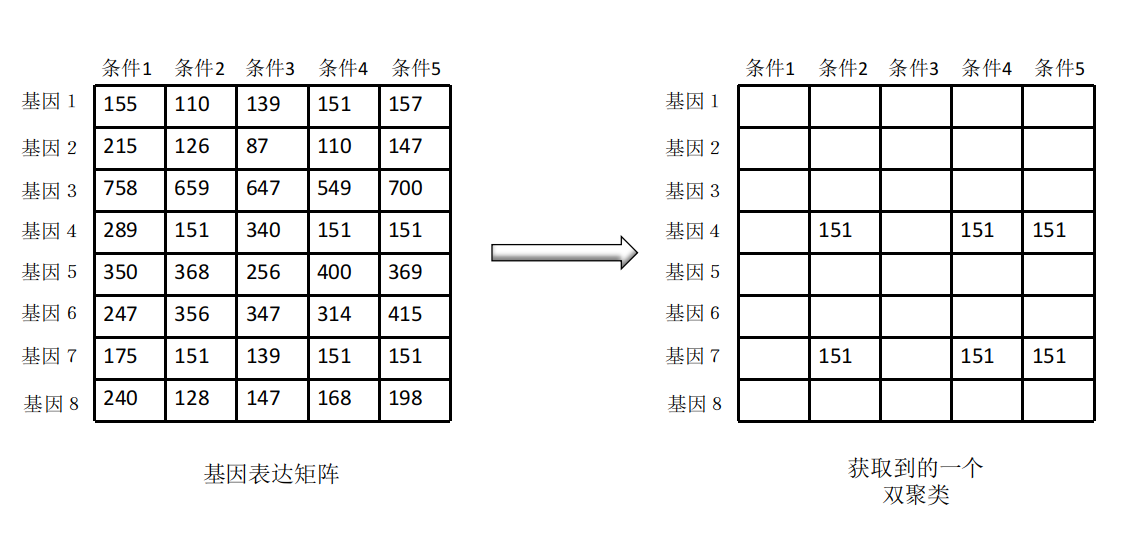
\includegraphics[width = 0.8\textwidth]{aBicluster.png}
  \caption{双聚类定义示例}
  \label{fig:define_bic}
  \end{figure}

  \subsection{双聚类的类型}
  给定一个二维矩阵$A(I,J)$,$a_{ij}$为其中第$i$行第$j$列的值,$\alpha_i$是一个与行有关而与列无关的变量,$\beta_j$是一个与列有关而与行无关的变量,$0\le h,r,t,d \le |I|$或$0\le h,r,t,d \le |J|$。Madeira 和 Oliveira提出,在双聚类中主要有以下四种类型:
  \begin{enumerate}
    \item[1.] 具有相同常量值的双聚类。该类型的双聚类所有的元素为同一个常量,如图\ref{bic61}所示,公式如下。
    \begin{equation}
      a_{ij}=\mu
    \end{equation}

    \item[2.] 列或行具有相同常量值的双聚类,满足公式\ref{equ:hang}的双聚类属于行常量值双聚类,如图\ref{bic62}所示。满足公式\ref{equ:lie}的双聚类属于列常量值双聚类,如图\ref{bic63}所示。
    \begin{equation}\label{equ:hang}
    a_{ij}=\mu+\alpha_i \mbox{或} a_{ij}=\mu *\alpha_i 
    \end{equation}
    \begin{equation}\label{equ:lie}
    a_{ij}=\mu+\beta_j  \mbox{或} a_{ij}=\mu *\beta_j
    \end{equation}
    
    \item[3.] 数值一致的双聚类,如图\ref{bic64}和\ref{bic65}所示,满足的公式如下。
    \begin{align}
    a_{ij}=\mu+\alpha_i+\beta_j \label{equ:jiafa}\\
    a_{ij}=\mu *\alpha_i*\beta_j\label{equ:chengfa}
    \end{align} 

    \item[4.] 具有连贯演变的双聚类,如图\ref{bic66}所示,公式如下。
    \begin{align}
    a_{ih}\le a_{ir}\le a_{it}\le a_{id} \\
    a_{hj}\le a_{rj}\le a_{tj}\le  a_{dj} 
    \end{align}
  \end{enumerate}

  \begin{figure}[htbp]
  \setlength{\subfigcapskip}{-1bp}
  \centering
  \begin{minipage}{.7\textwidth}
  \centering
  \subfigure{\label{bic61}}\addtocounter{subfigure}{-2}
  \subfigure{\subfigure[]{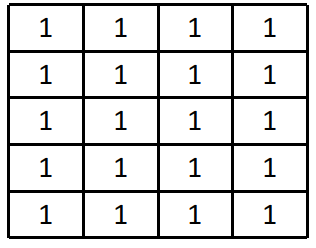
\includegraphics[width=0.3\textwidth]{a-bic}}}
  \hspace{.2em}
  \subfigure{\label{bic62}}\addtocounter{subfigure}{-2}
  \subfigure{\subfigure[]{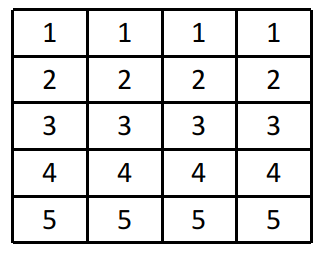
\includegraphics[width=0.3\textwidth]{b-bic}}}
  \hspace{.2em}
  \subfigure{\label{bic63}}\addtocounter{subfigure}{-2}
  \subfigure{\subfigure[]{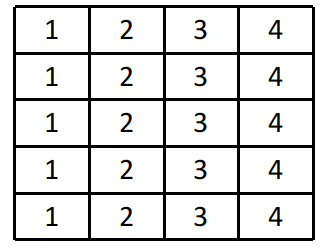
\includegraphics[width=0.3\textwidth]{c-bic}}}
  \end{minipage}
  \centering
  \begin{minipage}{.7\textwidth}
  \centering
  \subfigure{\label{bic64}}\addtocounter{subfigure}{-2}
  \subfigure{\subfigure[]{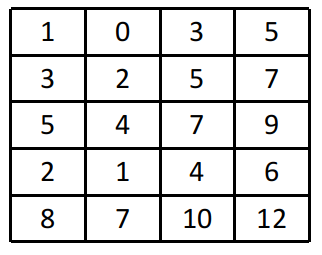
\includegraphics[width=0.3\textwidth]{d-bic}}}
  \hspace{.2em}
  \subfigure{\label{bic65}}\addtocounter{subfigure}{-2}
  \subfigure{\subfigure[]{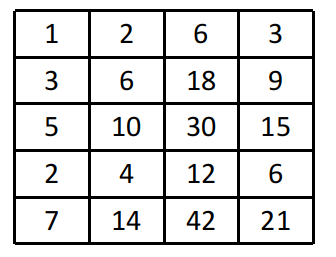
\includegraphics[width=0.31\textwidth]{e-bic}}}
  \hspace{.2em}
  \subfigure{\label{bic66}}\addtocounter{subfigure}{-2}
  \subfigure{\subfigure[]{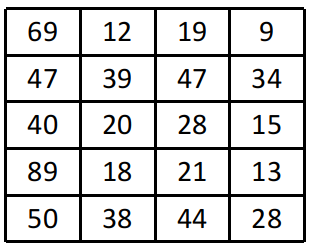
\includegraphics[width=0.3\textwidth]{f-bic}}}
  \end{minipage}
  \vspace{0.2em}
  \caption{双聚类的类型}
  \end{figure}

  \subsection{双聚类的结构}
  双聚类的结构是指,通过算法找到的双聚类之间在原始矩阵时间的相对位置。根据结构,大体可以分为8类:
  \begin{figure}[!h]
  \setlength{\subfigcapskip}{-1bp}
  \centering
  \begin{minipage}{.8\textwidth}
  \centering
  \subfigure{\label{bic81}}\addtocounter{subfigure}{-2}
  \subfigure{\subfigure[单一结构]{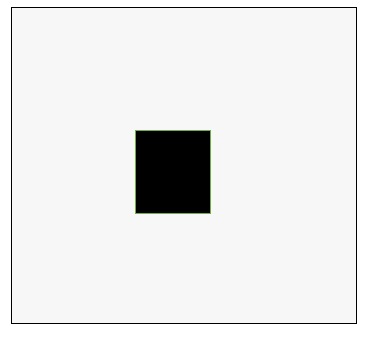
\includegraphics[width=0.2\textwidth]{struct1}}}
  \hspace{.2em}
  \subfigure{\label{bic82}}\addtocounter{subfigure}{-2}
  \subfigure{\subfigure[对角结构]{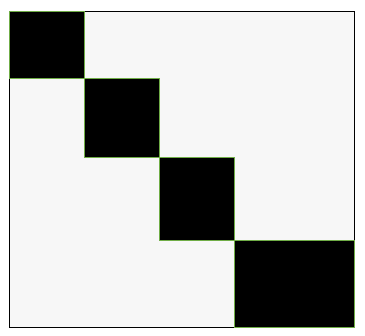
\includegraphics[width=0.2\textwidth]{struct2}}}
  \hspace{.2em}
  \subfigure{\label{bic83}}\addtocounter{subfigure}{-2}
  \subfigure{\subfigure[棋盘结构]{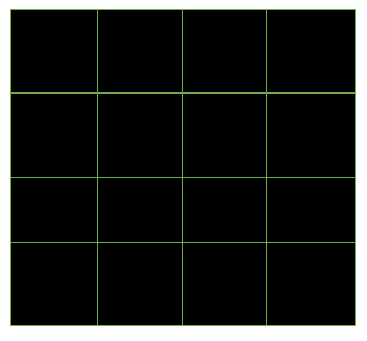
\includegraphics[width=0.2\textwidth]{struct3}}}
  \hspace{.2em}
  \subfigure{\label{bic84}}\addtocounter{subfigure}{-2}
  \subfigure{\subfigure[行互斥结构]{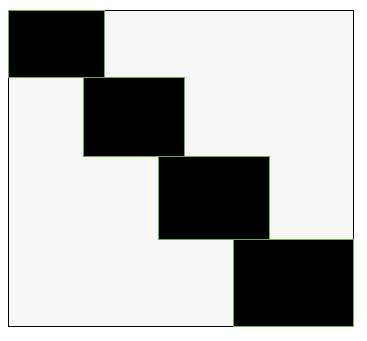
\includegraphics[width=0.2\textwidth]{struct4}}}
  \end{minipage}
  \centering
  \begin{minipage}{.8\textwidth}
  \centering
  \hspace{.2em}
  \subfigure{\label{bic85}}\addtocounter{subfigure}{-2}
  \subfigure{\subfigure[列互斥结构]{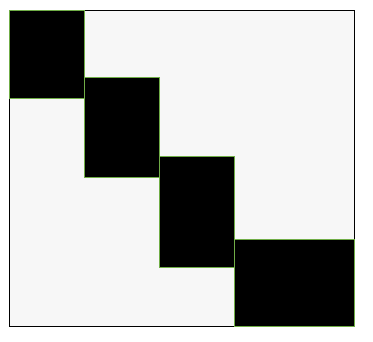
\includegraphics[width=0.2\textwidth]{struct5}}}
  \hspace{.2em}
  \subfigure{\label{bic86}}\addtocounter{subfigure}{-2}
  \subfigure{\subfigure[非互斥且非重叠结构]{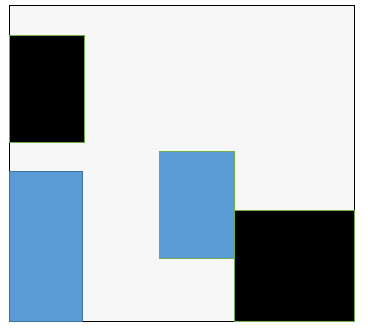
\includegraphics[width=0.2\textwidth]{struct6}}}
  \hspace{.2em}
  \subfigure{\label{bic87}}\addtocounter{subfigure}{-2}
  \subfigure{\subfigure[嵌套重叠结构]{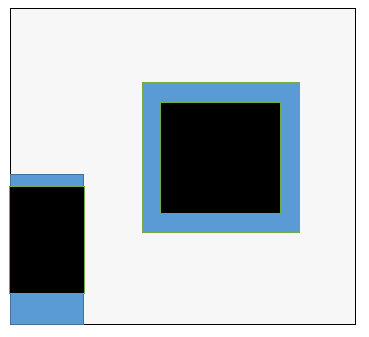
\includegraphics[width=0.2\textwidth]{struct7}}}
  \hspace{.2em}
  \subfigure{\label{bic88}}\addtocounter{subfigure}{-2}
  \subfigure{\subfigure[任意重叠结构]{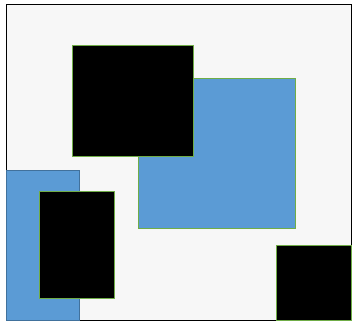
\includegraphics[width=0.2\textwidth]{struct8}}}
  \end{minipage}
  \vspace{0.2em}
  \caption{双聚类的结构}
  \label{fig:bic-struct}
  \end{figure}
  \begin{enumerate}
    \item[(1)] 单一结构。指基因表达数据中只存在一个双聚类,且基因和条件可以不属于该双聚类,如图\ref{bic81}所示。
    \item[(2)] 对角结构。指任意两个双聚类之间互不共享行和列,且任一行或列只能属于其中一个双聚类,如图\ref{bic82}所示。这类的双聚类可以通过交换位置,最后呈对角线形状。
    \item[(3)] 棋盘结构,指通过传统的聚类方法分别对行和列进行聚类,然后组合得到的双聚类,如图\ref{bic83}所示。
    \item[(4)] 行互斥结构。指双聚类之间不存在共享的行,可以看作有对角线结构放松对行的限制所得,如图\ref{bic84}所示。
    \item[(5)] 列互斥结构。与行互斥相似,指双聚类之间不存在共享的列,如图\ref{bic85}所示。
    \item[(6)] 非互斥且非重叠结构。之允许双聚类之间存在相同的行或列,但不能存在重叠和包含关系,如图\ref{bic86}所示。
    \item[(7)] 嵌套重叠结构。指双聚类之间可以存在包含关系,但不能出现重叠关系,如图\ref{bic87}所示。
    \item[(8)] 任意重叠结构。指双聚类之间即可以存在包含关系,也可以存在重叠关系,如图\ref{bic88}所示。
  \end{enumerate}

  传统的聚类只能找到像图\ref{bic81}所示的单一结构,这对于基因表达数据的挖掘是远远不够的。嵌套和重叠的结构要比非嵌套和非重叠的结构复杂,需要更复杂的算法来找到它们。

  
\section{双聚类的评价指标}
  \subsection{质量评价指标}\label{section:qualityEval}
  由于在基因表达数据进行双聚类分析是NP难问题,目前大部分的算法都是基于优化策略的。为了评价双聚类的质量和知道优化的方向,需要有效的评价指标。指标是否科学可靠直接会体现到双聚类结果上。本节对目前常用的评价指标进行一个总结。
  
  方便起见,先引入一些数学定义。给定一个大小为$n\times m$的基因表达数据$E(X,Y)$,以及一个大小为$k\times l$的双聚类$B(I,J)$,$b_{Ij}$为$B$中第$j$列的平均值,$b_{iJ}$为$B$中第$i$行的平均值,$b_{IJ}$为双聚类整体的平均值,$Vol_B$表示双聚类的体积,公式定义如下:
  \begin{align}
    b_{iJ} &= \sum_{j\in J}\frac{b_{ij}}{|J|} \\
    b_{Ij} &= \sum_{i\in I}\frac{b_{ij}}{|I|} \\
    b_{IJ} &= \sum_{i\in I,j\in I}\frac{ b_{ij} }{|I| \times |J|}\\
    Vol_B &= |I| \times |J|
  \end{align}
  \begin{enumerate}
    \item[(1)] 方差。用$Var(B)$表示双聚类$B(I,J)$的方差,该指标代表了该双聚类的变化幅度,越大则双聚类中的值越不相同,定义如下:
    \begin{equation}
      Var(B) = \sum_{i\in I,j\in I}\frac{(b_{ij}-b_{IJ})^2}{Vol_B}
    \end{equation}

    \item[(2)] 均方残差。该指标首先在CC算法中提出,并被广泛地应用在基因表达矩阵的分析中。数学定义如公式\ref{equ:msr}所示。该指标适合寻找像式\ref{equ:jiafa}这样的加法模型双聚类,且值越小越符合该模型。
    \begin{equation}\label{equ:msr}
      MSR(B) = \frac{1}{Vol_B}\sum_{i=1}^k\sum_{j=1}^l(b_{ij}-b_{iJ}-b_{Ij}+b_{IJ})^2
    \end{equation}

    \item[(3)] 扩展均方残差。因为$MSR(B)$只能发现加法模型,Mukhopadhyay 等提出了扩展均方残差(Scaling Mean Squared Residue,SMSR)。该指标适合寻找如\ref{equ:chengfa}这类的乘法模型双聚类,且值越小越符合该模型。双聚类$B(I,J)$的SMSR(B)定义如下:
    \begin{equation}\label{equ:smsr}
      SMSR(B) = \frac{1}{Vol_B}\sum_{i=1}^k\sum_{j=1}^l(\frac{b_{iJ}\times b_{Ij}-b_{ij}\times b_{IJ}}{b_{iJ}\times b_{Ij}})^2
    \end{equation}

    \item[(4)] 相关指数。该指标用来寻找列值常量类型的双聚类,定义如下:
    \begin{equation}
      RI(B) = \sum_{j=1}^l R_{Ij}/l = \sum_{j=1}(1 - \frac{\sigma_{Ij}^2}{\sigma_j^2})/l
    \end{equation}
    \hspace{2em} 其中,$R_{Ij}$为双聚类中第$j$列的相关指数,$\sigma_{Ij}^2$是双聚类中第$j$列所有元素的局部方差,$\sigma_{j}^2$是基因表达数据第$j$列所有元素的全局方差。该指标越大则越符合列值常量类型。类似的,稍加改造则可以寻找行值常量类型的双聚类。

    \item[(5)] 最大标准化区域。该指标由Giraldez 等提出,并用于寻找趋势一致的双聚类。计算过程:首先要对双聚类$B(I,J)$进行标准化,得到$\hat{B}(I,J)$,计算公式为:
    \begin{equation}
      \hat{b}_{ij} = \frac{b_{ij}-b_{iJ}}{\sigma_i}
    \end{equation}
    \hspace{2em} 其中,$b_{iJ}$和$\sigma_i$为双聚类$B$中第$i$行元素的平均值和标准差。根据$\hat{B}(I,J)$,双聚类$B(I,J)$的最大标准化区域的定义如下:
    \begin{equation}
      MSA(B) = \sum_{j=1}^l \mid \frac{M_j-m_j-M_{j+1}+m_{j+1}}{2}\mid
    \end{equation}
    \hspace{2em} 其中,$M_j=max_{i\in [i,k]}\hat{b}_{ij}$,$m_j=min_{i\in [i,k]}\hat{b}_{ij}$。当双聚类中基因表达模型完全一致时,$MSA(B)=0$。

    \item[(6)] HV-Score。一个双聚类$B(I, J)$的Hv-Score定义如下:
    \begin{equation}
     Hv(B) = \frac{\sum_{i=1}^k \sum_{j=1}^l(b_{ij}-b_{iJ}-b_{Ij}+b_{IJ})^2}{\sum_{i=1}^k \sum_{j=1}^l(b_{ij}-b_{iJ})^2}
    \end{equation}
    该指标是对MSR的改进,改善了MSR偏向找到常量类型双聚类的不足,由Bryan等提出。值越小则双聚类的质量越好。

    \item[(7)] 覆盖率。该指标是双聚类集合的多样性指标,因为大多数算法找到的双聚类都不止一个,如果双聚类过度重合则意义不大。我们总是希望找到互相重叠小且能覆盖到更多的基因表达数据的双聚类集合。 假设双聚类集合$\Pi=\{B_1,B_2,...,B_r\}$,$\phi_k(E)$为判断$E(X,Y)$中每个元素$e_{ij}$是否在双聚类$B_k$的函数。定义公式如下:
    \begin{equation}
    \phi_k(a_{ij})  = \left\{
      \begin{aligned}
       1 & = & if a_{ij} \in B_k \\
       0 & = & otherwise 
      \end{aligned}
    \right.
    \end{equation}
  \end{enumerate}
  \hspace{2em}则双聚类集合$\Pi$的覆盖率$covRate(\Pi)$定义如下:
  \begin{equation}
   covRate(\Pi) = \frac{\sum_{i=1}^k\sum_{j=1}^l\cup_{k=1}^r\phi_k(a_i)}{n \times m} 
  \end{equation}
  \hspace{2em}从定义可以看出,覆盖率的含义是集合$\Pi$中$r$个子矩阵并集所占基因表达数据$E$的比例。

  \subsection{生物评价指标}
  为了评价通过双聚类获得基因集合的生物意义,需要对其进行基因解释。生物技术的发展积累了很多关于基因的描述,这些信息可以为我们提供参考。目前,最流行的基因注释数据库当属KEGG数据库和GO数据库。前者主要用来做旁路分析,所谓旁路分析,就是获得基因之间的调控关系,后者主要用来做富集分析,对基因功能进行注释。目前对双聚类结果的生物验证主要还是GO的富集分析。

  GO数据库中保存了各种物种的基因的注释信息,包括基因的功能和之间的关系。GO将基因的功能分为分子功能(Molecular Funciotn,MF),细胞组成(Cell Compose,CC)和生物过程(Biological Process,BP)。GO将一项功能称为一个GO项(term),并通过一个有向无环图表示项与项之间的关系。如果两个GO项之间有连线,则表示之间存在联系。如果双聚类中关于某一GO项的基因个数大于该项随机概率出现的次数,则称该双聚类的基因集合富集在这一GO项,并用通过统计学方法,得到统计值P-value来表示富集的程度。P-value越小,则富集程度越大,一般只关注P-value小于0.01的GO项。  
  \begin{enumerate}
    \item[(1)] 显著富集双聚类的比例。对于双聚类集合$\Pi=\{B_1,B_2,...,B_r\}$,假设其中存在$r_{sig} \le r$个双聚类存在富集。显著富集双聚类的比例(Proportion of the biclustersSignificantly Enriched, proSigEnriched)定义如下:
    \begin{equation}
      proSigEnriched = \frac{r_{sig}}{r} \times 100\%
    \end{equation}

    \item[(2)] 带权重的富集分数。$proSigEnriched$只是在双聚类层面的验证指标,不仅没有精确到功能项而且对于基因集合很大的双聚类很难区分。所以,带权重的富集分数(Weight Enrichment Score, WEScore)被引入进来,定义如下:
    \begin{equation}\label{equ:wescore}
      WEScore = \sum_{i=1}^t{x_i s_i}/k
    \end{equation}
    \hspace{2em}其中,$t$是双聚类$B$经过GO分析后得到的GO项的个数,$x_i$是对应第$i$个GO项的基因个数,$s_i$是对应GO项经过负对数变换后的P值,$k$是双聚类中基因的个数。$WEScore(B)$越大则该双聚类生物意义越大。

    \item[(3)] 平均P值。与$WEScore$类似,平均P值(Mean of P Values, meanPValue)的定义如下:
    \begin{equation}\label{equ:meanP}
      meanPValue = \sum_{i=1}^ts_i/t
    \end{equation}
    \hspace{2em}其中,$t$与$s_i$与公式\ref{equ:wescore}含义一样,且$meanPValue(B)$越大则该双聚类生物意义越大。

    \item[(4)] 基因与GO项的比值。由于一个双聚类一般会在很多个GO项出现富集,如果GO项的个数越少,则说明双聚类中的基因之间越相关。因此,引入了基因与GO项的比值(Ratio of number of gene to number of significant terms, rateGeneTerm),定义如下:
    \begin{equation}
     rateGeneTerm(B) = k / t 
    \end{equation}
    \hspace{2em}其中,$k$和$t$与公式\ref{equ:wescore}中含义一致。
  \end{enumerate}

\section{双聚类算法的分类}
  \subsection{基于质量评价的双聚类算法}
  因为在基因表达数据上进行双聚类分析是NP难问题,所以无法通过穷举的方式来搜索双聚类。上一节给出了一些质量评价指标,大部分算法都是使用不同的策略,找到在一种或多种评价指标最优的双聚类。根据搜索策略的不同,可以将算法分为以下几类。
  \begin{enumerate}
    \item[(1)] 基于贪婪迭代搜索策略。这类算法,一般是从一个初始的双聚类出发,然后根据质量指标迭代地添加或移除基因或条件节点。该类算法的有点是速度快,但通常质量欠佳。MSB(Maximum Similarity Biclusters)算法以及CC算法就其中的典型算法。

    \item[(2)] 基于随机贪婪搜索。如前一种不同的是,此类算法在迭代过程中并不只考虑最优的操作,而是一定概率采取次优的操作,保证了搜索的多样性。FLOC算法就属于此类。
    
    \item[(3)] 基于聚类算法。该类算法的特点是,先使用传统的聚类方法分别对行和列进行聚类,并将其组合起来,然后在组合得到的双聚类中挑取质量评价较好的结果。例如,PSB算法先使用IPC聚类算法在行和列两个方向聚类分析,然后使用MSR(B)筛选组合后得到的双聚类。
    
    \item[(4)] 基于元启发式算法。元启发算法的特点是模拟大自然中生物的高效的搜索行为,例如例子群算法,蚁群算法。这类算法通过使用双聚类的质量评价指标组合成适应度函数,从而找到质量评价指标高的双聚类。
  \end{enumerate}

  \subsection{基于模型的双聚类算法}
  在有些双聚类算法中,并没有使用质量评价指标,该类算法被成为基于模型的双聚类算法。如基于图论的SAMBA算法,基于概率模型的Plaid算法,基于矩阵论的ISA算法,基于排序的OPSM算法,基于关联规则挖掘的BiModule算法。TODO

\section{群智能算法}
目前,有很多优秀的优化算法,有确定性方法如线性规划、二次规划,动态规划和梯度下降;以及随机性方法如群体智能。这些方法让我们能够在一定的时间内解决某些问题。然而,处理大量高维数据时,确定性方法太过复杂导致需要大量的计算成本。元启发式的群体智能算法因其高效率越来越受到关注。

  \subsection{粒子群算法}
  粒子群(Particle Swarm Optimization,PSO)算法是Kennedy和Eberhart于1995年提出的一种群体智能优化算法,流程图如图\ref{fig:pso}所示。该算法是受到了鸟群觅食过程中的集体行为的启发。PSO 算法将群体中的粒子看作可行域中的一个点,这些点既没有质量也没有体积,只有一定的初始速度,在可行域中飞行。粒子可以通过飞行过程中自身的最优值和群体的最优值不断地修正自己的前进方向和速度大小,从而形成群体寻优的正反馈机制。其粒子更新方式为:
  \begin{align}
    &v_i= wv_i +c_1r_1(pbest_i-x_i )+c_2r_2(gbest-x_i )\\
    &x_{i} = x_i+v_i 
  \end{align}
  其中, $v_i$是粒子$i$的速度矢量, $x_i$ 是粒子$i$的位置矢量,$pbest$是粒子$i$的历史中最优的位置。$gbest$是所有粒子的历史中最优的位置。$c_1,c_2$是加速度常数,调节学习最大步长。 $r_1,r_2$是两个随机函数,取值范围[0,1],以增加搜索随机性。 $w$是惯性权重,非负数,调节对解空间的搜索范围。

  粒子速度更新公式包含三部分: 第一部分为“惯性部分”,即对粒子先前速度的记忆;第二部分为“自我认知”部分,可理解为粒子i当前位置与自己最好位置之间的距离;第三部分为“社会经验”部分,表示粒子间的信息共享与合作,可理解为粒子i当前位置与群体最好位置之间的距离。
  \begin{figure}[htbp]
    \centering
    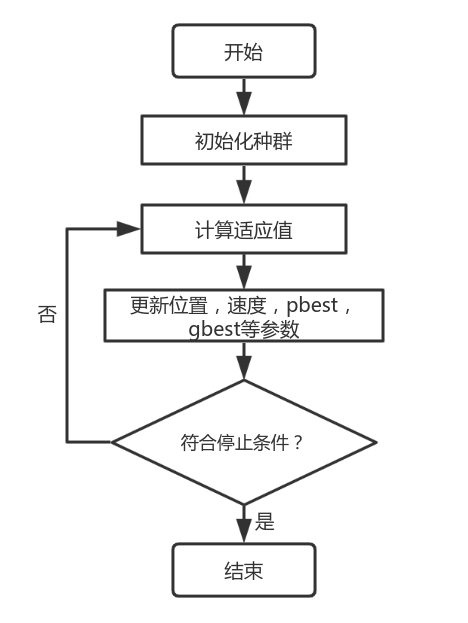
\includegraphics[width = 0.5\textwidth]{pso}
    \caption{粒子群算法流程图}
    \label{fig:pso}
  \end{figure}

  \subsection{布谷鸟搜索算法}
    布谷鸟搜索算法(Cuckoo Search, CS)是Yang和Deb于2009年提出的新兴启发算法,流程图如图\ref{fig:cs}所示。该算法通过模拟布谷鸟寄生育雏行为,在可行域中通过Levy飞行寻找合适的鸟巢,来找到较优解。该算法有三条理想化的规则:
    \begin{enumerate}
      \item {每只布谷鸟每次下一个蛋,并将其放入随机选择的巢中。}
      \item {具有优质蛋的最佳巢会被带到下一代。}
      \item {可用的寄主巢数量是固定的,且寄主以概率$P_a\in(0,1)$发现布谷鸟放的蛋。在这种情况下,寄主可以消灭该蛋或放弃旧巢另建新巢。}
    \end{enumerate}

    CS中有两种更新方式,一种是布谷鸟寻找宿主鸟巢的Levy飞行:
    \begin{align}
      x_{i+1}=x_i+\alpha\otimes Levy(\beta)
    \end{align}
    其中,$\alpha$是步长缩放因子, $Levy(\beta)$是Levy飞行路径。

    另一种是寄主以概率$P_a$发现外来鸟蛋后,采用随机方式重新建巢:
    \begin{equation}
      x_{i+1}=x_i+r\otimes Heaviside(P_a-\varepsilon)\otimes(x_t-x_k)
    \end{equation}
    其中,$r,\varepsilon$是服从均匀分布的随机数,$Heaviside()$是跳跃函数,$x_t,x_k$是其他任意的两个鸟巢。
    \begin{figure}[htbp]
      \centering
      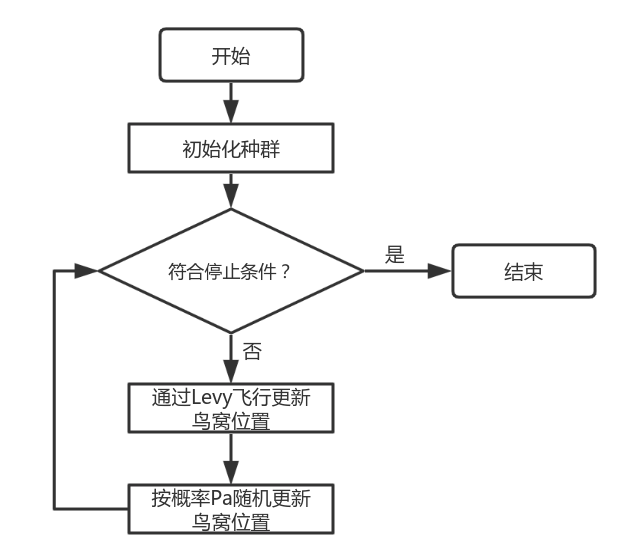
\includegraphics[width = 0.7\textwidth]{cs}
      \caption{布谷鸟算法流程图}
      \label{fig:cs}
    \end{figure}

  \subsection{萤火虫算法}
  萤火虫算法(Firefly Algorithm,FA)是Yang于2008年提出的一种启发算法,流程图如图\ref{fig:fa}所示。把空间各点看成萤火虫,利用发光强的萤火虫会吸引发光弱的萤火虫的特点,在发光弱的萤火虫向发光强的萤火虫移动的过程中,完成位置的迭代,从而找出最优位置。算法有以下三条假设:
  \begin{enumerate}
    \item {萤火虫不分性别,这样一个萤火虫将会吸引到所有其他的萤火虫。}
    \item {吸引力与它们的亮度成正比,对于任何两个萤火虫,不那么明亮的萤火虫被吸引,因此移动到更亮的一个,然而,亮度又随着其距离的增加而减少。}
    \item {如果没有比一个给定的萤火虫更亮的萤火虫,它会随机移动。}
  \end{enumerate}
  萤火虫的相对荧光亮度计算方式:
  \begin{align}
    I=I_0e^{-\gamma r_{ij}}
  \end{align}
  其中, $I_0$表示最亮萤火虫的亮度,即自身($r=0$处)荧光亮度,与目标函数值相关,目标函数值越优,自身亮度越高;$\gamma$表示光吸收系数,因为荧光会随着距离的增加和传播媒介的吸收逐渐减弱,所以设置光强吸收系数以体现此特性,可设置为常数;$r_{ij}$表示萤火虫$i$与$j$之间的距离。 

  当萤火虫$i$的相对亮度小于萤火虫$j$时,向萤火虫$j$靠拢。位置的更新方式为:
  \begin{align}
    \beta(r)&=\beta_0e^{-\gamma r_{ij}^2} \\
    x_i&=x_i+\beta(x_j-x_i)+\alpha(rand-1/2)
  \end{align}
  其中, $\beta_0$表示最大吸引度,即光源处($r=0$处)的吸引度。$\alpha$为步长因子,$rand$为[0,1]上服从均匀分布的随机因子。

  \begin{figure}[htbp]
    \centering
    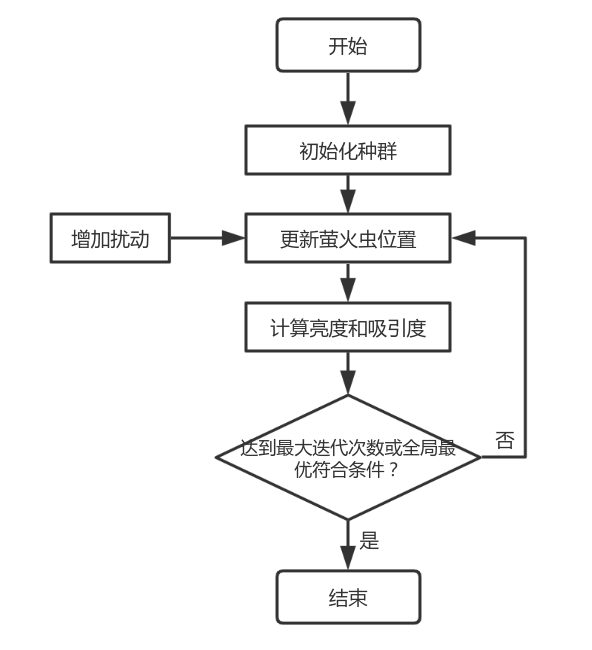
\includegraphics[width = 0.6\textwidth]{fa}
    \caption{萤火虫算法流程图}
    \label{fig:fa}
  \end{figure}

  \subsection{细菌觅食算法算法}
  细菌觅食算法算法(Bacterial Foraging Optimization,BFO)由Passino于2002年提出,流程图如图\ref{fig:bfo-2}所示。通过模拟大肠杆菌菌落的觅食行为,不断地使用鞭毛游动和翻转,最终躲开有毒的地方并找到营养度高的位置,如图\ref{fig:bfo}所示。算法分为趋向性操作(趋化操作)、复制操作和迁徙操作。
  \begin{figure}[htbp]
    \centering
    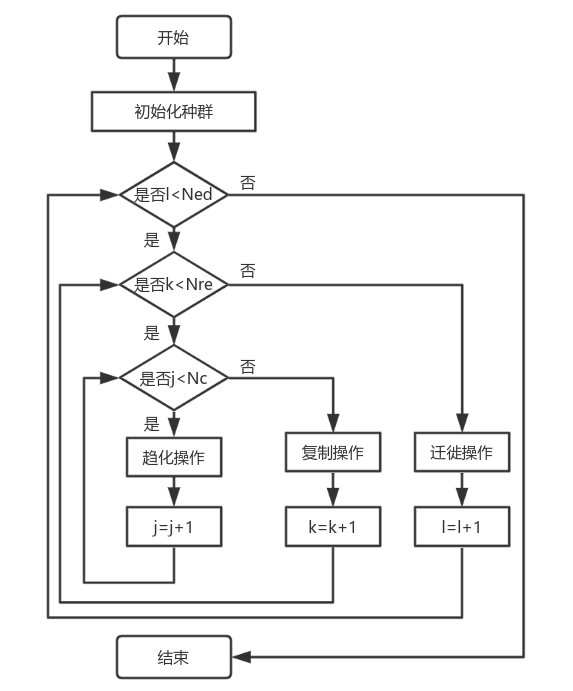
\includegraphics[width = 0.5\textwidth]{bfo-2}
    \caption{细菌觅食算法流程图}
    \label{fig:bfo-2}
  \end{figure}
  
  \begin{figure}[htbp]
    \centering
    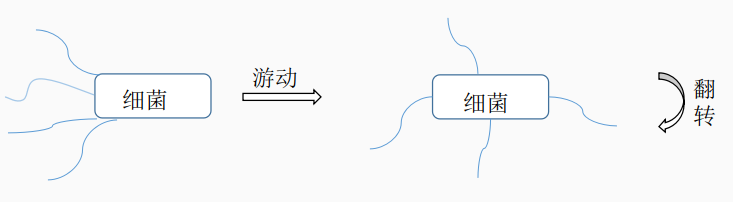
\includegraphics[width = 0.7\textwidth]{bfo.png}
    \caption{细菌的游动和翻转}
    \label{fig:bfo}
  \end{figure}

  \begin{enumerate}
    \item[1.] 趋向性操作。 
    这一操作模拟得是大肠杆菌的游动和翻转。在营养度高的地区,细菌会更多地游动,在营养度低的地区,细菌会更多地翻转,以逃出该地区。设细菌的种群规模为$S$,维度为$n$。细菌的觅食行为可以用以下公式表示:
    \begin{align}
      \theta(i,j+1,k,l) &= \theta(i,j,k,l) + C(i) \times \phi(i,j) \\
      \phi(i,j) &= \frac{\Delta(i)}{\sqrt{\Delta^T(i)\Delta(i)}}
    \end{align}
    其中,$\theta(i,j,k,l)$表示细菌在第$j$次趋向性操作,第$k$次复制操作和第$l$次迁徙操作时的位置。$C(i)$是细菌$i$的趋向性步长。$\phi(i,j)$表示细菌在第$j$次趋向性操作时的随机方向的单位向量。$\Delta(i)$为随机向量。

    \item[2.] 复制操作。
    复制操作的目的是将表现不好的细菌淘汰掉。首先,对种群按适应度排序,然后,前一半的细菌会复制一份覆盖后一半的细菌。保持种群数量不变的同时,实现优胜劣汰的机制。

    \item[3.] 迁徙操作。
    在生物观察中发现,随着某些条件的改变,可能会使该地区的细菌突然死亡或迁移。算法通过迁徙操作模拟这一现象,提高种群的多样性。细菌会以一定的概率被清除,并随机生成一个新的细菌。
    
  \end{enumerate}

\section{本章小结}
生物信息学中,通过双聚类分析对基因表达数据进行挖掘,希望找到在对应条件下紧密相关的基因集合。本章主要对基因表达数据上的双聚类的相关知识进行了阐述,先是介绍了基因表达数据的重要以及特点;然后对双聚类的定义、类型和结构进行了描述;接下来对常用的质量评价指标以及生物评价指标进行了简要介绍,以及把双聚类算法分为了基于质量评价指标的和基于模型的两种;最后简要说明了本文用到的几种群智能算法。